\section{System Visualisation}
In this section, we provide a comprehensive visualization of the property management system by summarizing and displaying various diagrams. These diagrams are essential to show the structure, interactions and dynamic processes of the system in a clear and understandable way. By visualizing the system components and their relationships, we can gain a deeper understanding of how the system works and its architecture.
\subsection{ER-diagram}
An entity-relationship diagram (ER diagram) is an essential tool in system development that visually represents the data structure of a system. The ER diagram is particularly important for a real estate management system, as it illustrates the relationships between the various data entities and thus provides a basis for the design and implementation of the database schema.
\begin{figure}[h]
\centering
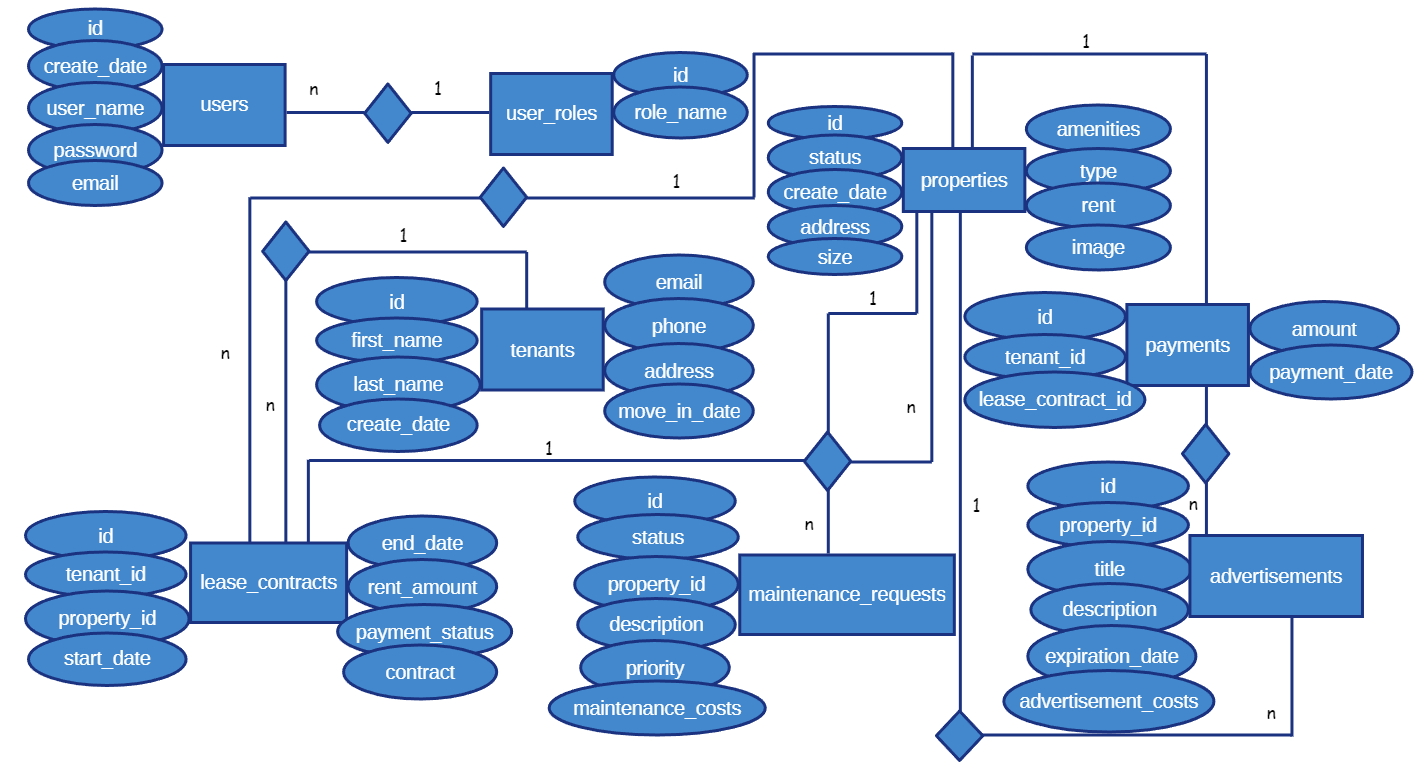
\includegraphics[height=10.50cm]{ER-Diagram.png}
\caption{ER-Diagram}
\label{fig:ER-Diagram}
\end{figure}

\newpage
\subsection{Use case diagram}
The use case diagram for the property management system provides a comprehensive overview of the various interactions between the user and the system. This diagram is an essential tool to visualize the functional requirements of the system. Each use case represents a unit of functionality that provides added value for users.
\begin{figure}[h]
\centering
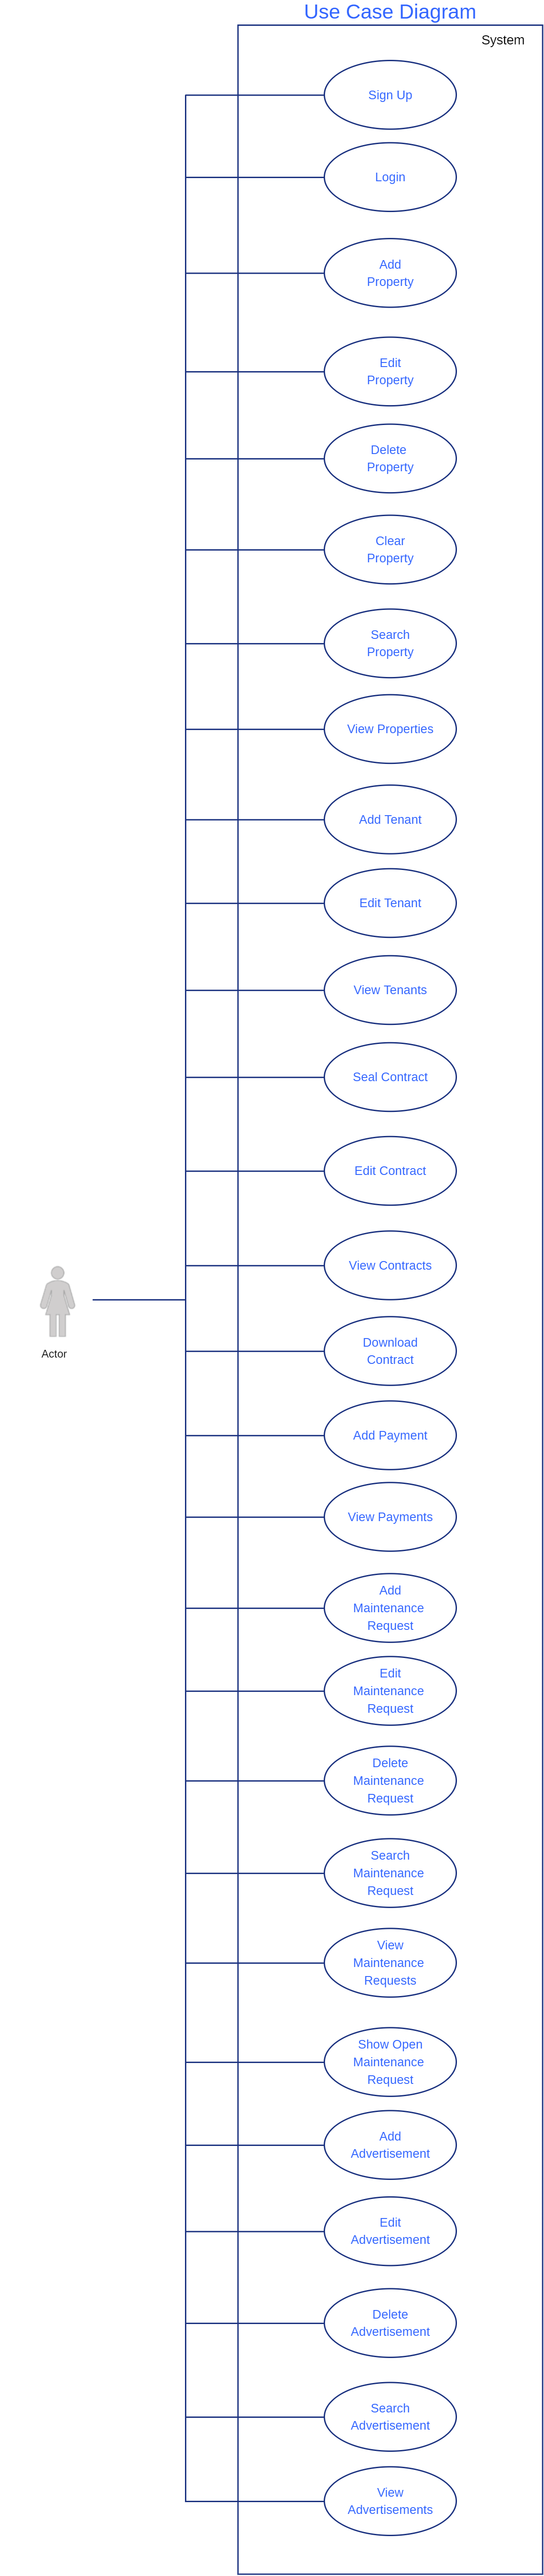
\includegraphics[height=16.50cm]{usecasediagram.png}
\caption{Use Case Diagram}
\label{fig:use-case-diagram}
\end{figure}

\newpage
\subsection{Class diagram}
The class diagram of the property management system represents the static structure of the system by describing the most important classes and their relationships to each other. It is a central modeling element in object-oriented software development and provides a detailed overview of the system architecture.

In the context of the property management system, the class diagram helps to visualize the various data objects, their attributes and methods as well as the interactions between them. This diagram forms the basis for the design and implementation of the software, as it defines the structure and logical relationships within the system.
\begin{figure}[h]
\centering
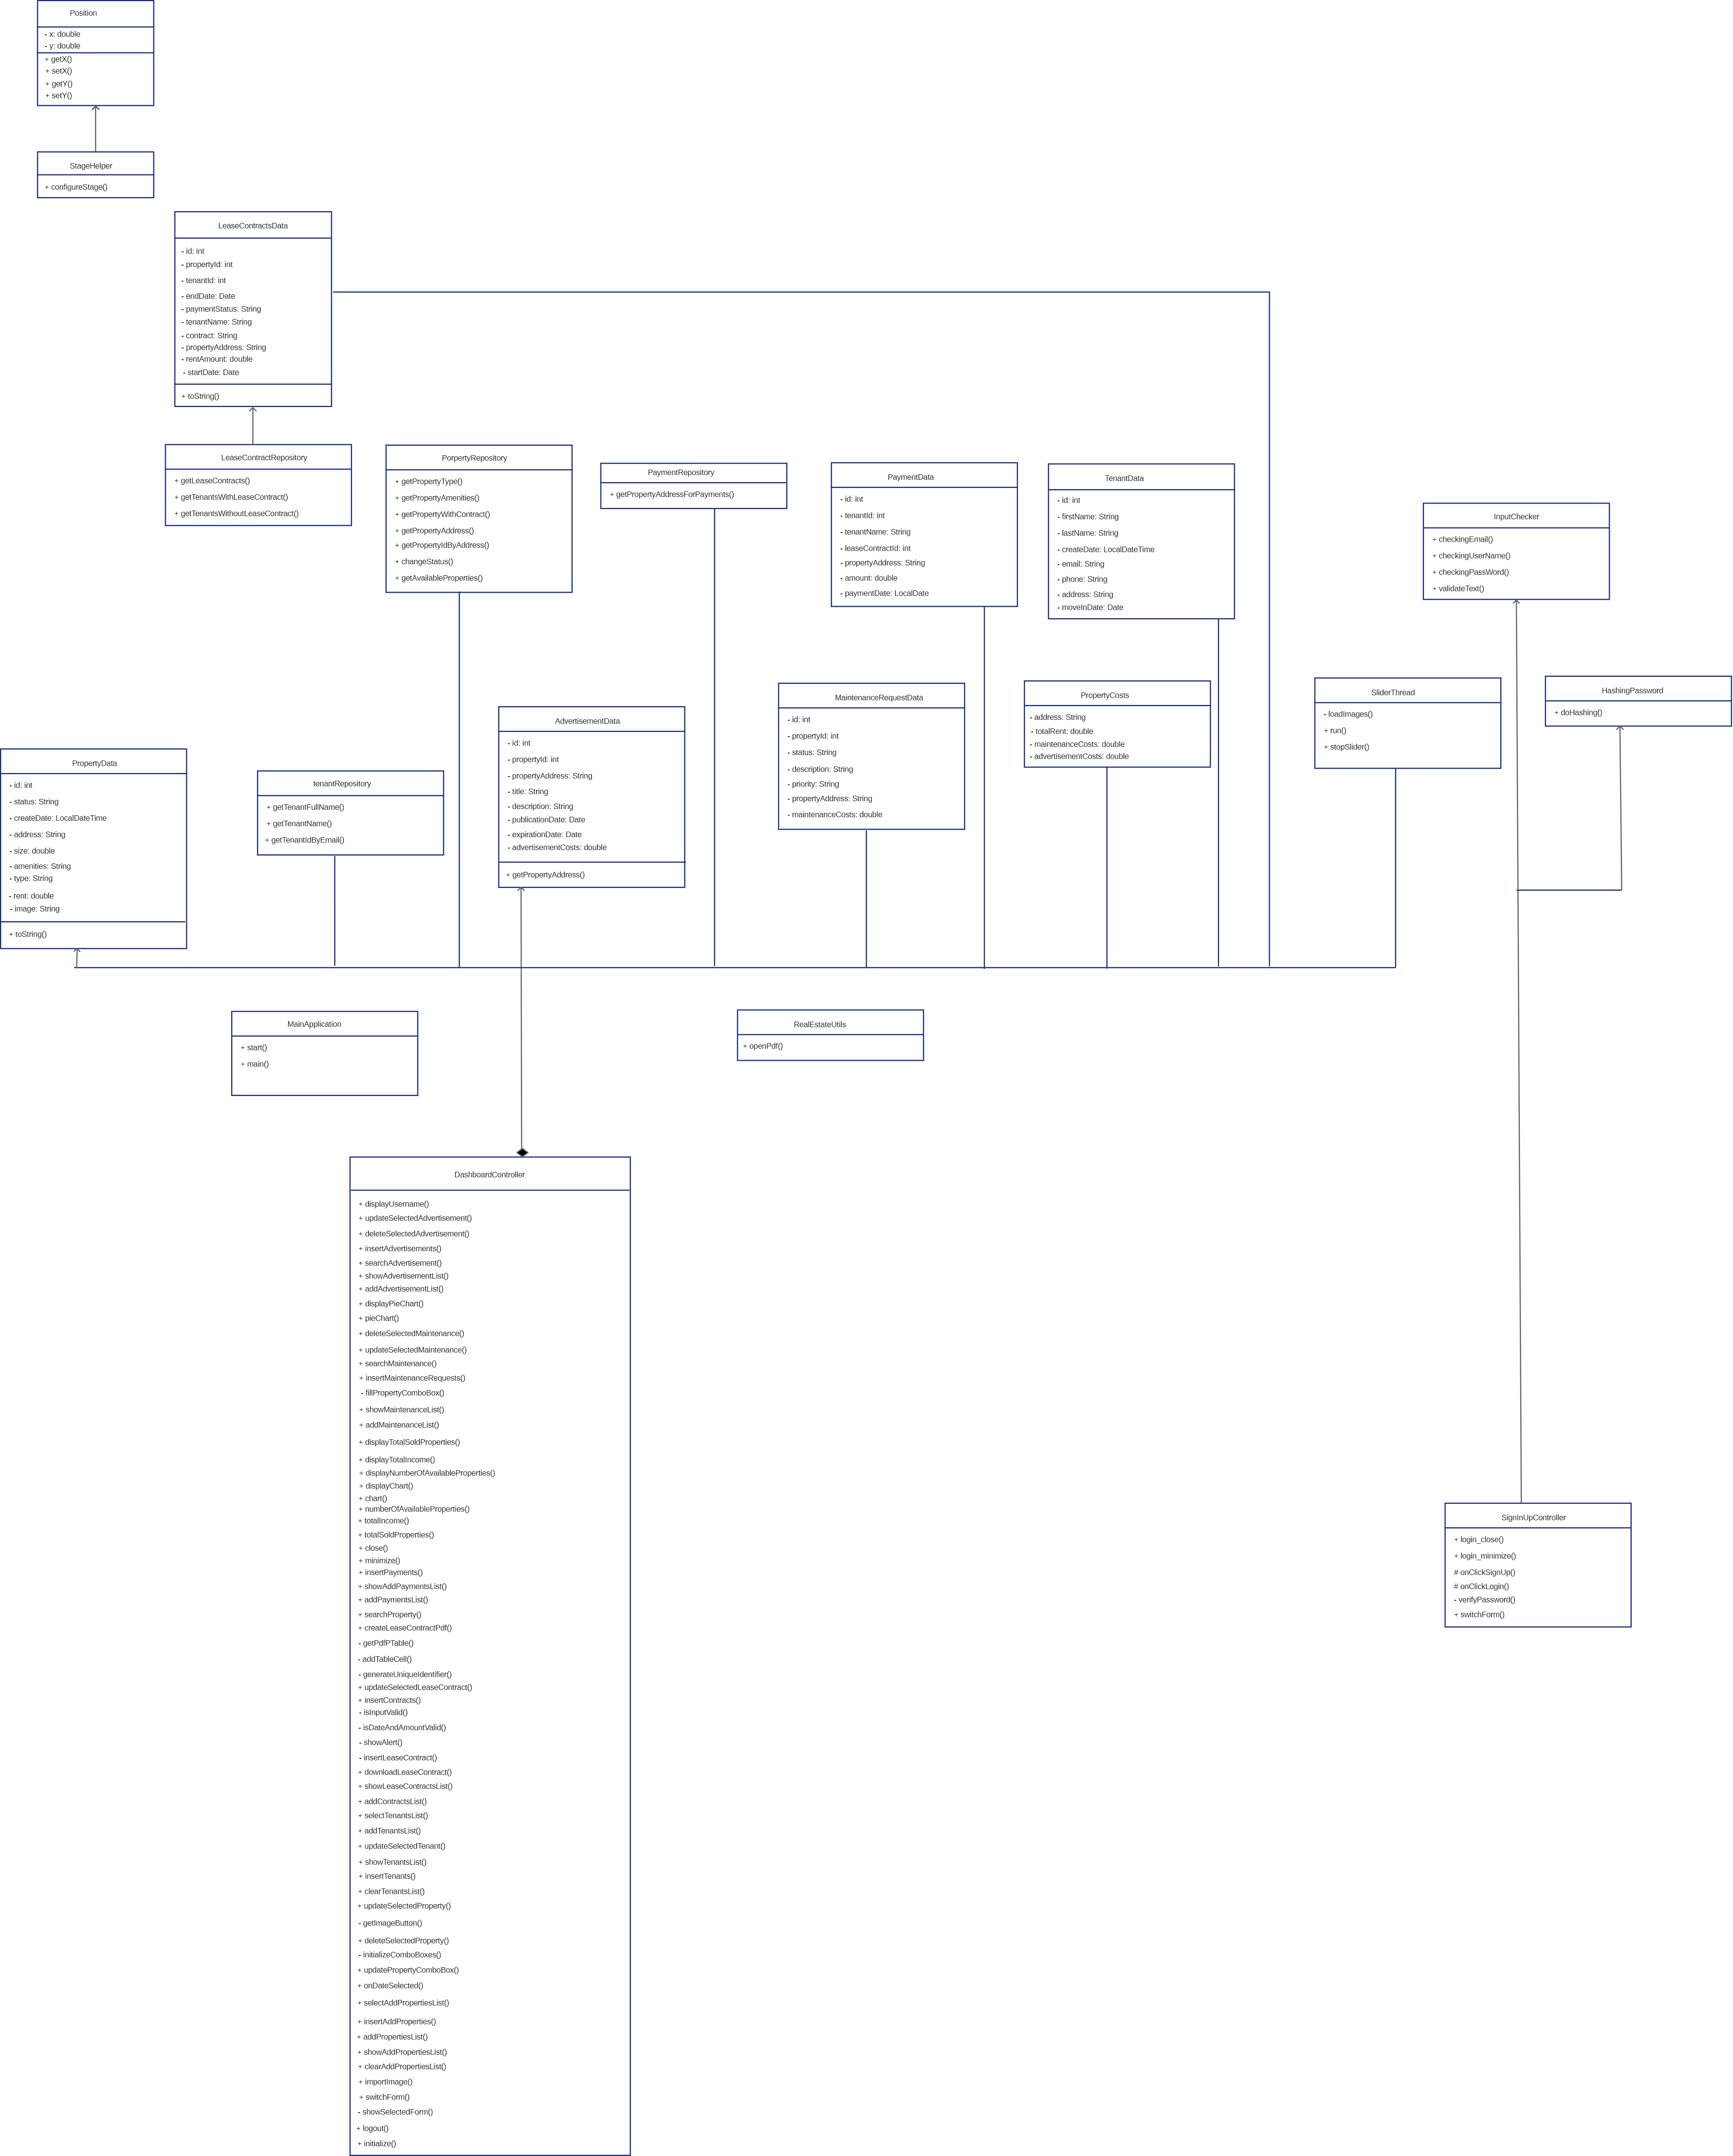
\includegraphics[height=16.50cm]{classdiagram.png}
\caption{Class Diagram}
\label{fig:class-diagram}
\end{figure}